% paladins

\pagebreak
\subsection{Paladins}


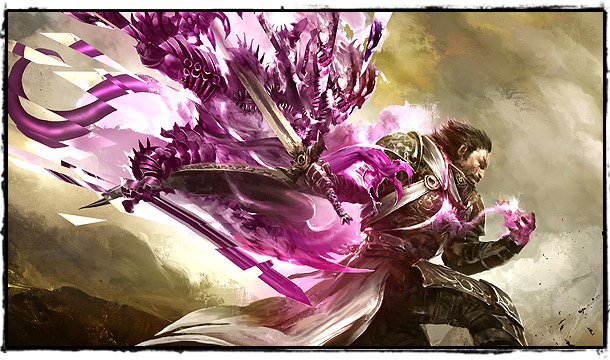
\includegraphics[width=\textwidth,height=\textheight,keepaspectratio]{paladin.jpg}

Paladins are holy warriors. They are specialized in the eradication of evil like demons and undead. There are three paths a paladin can follow and every level they gain they should choose one spell from that level of any path. 
Level 5 is a big step in the paladin's abilities. At level 5 you select a specialization. Choosing this specialization unlocks perks you can choose from within the \emph{tree of perks}.

Every paladin starts with the following three spells:

\begin{itemize}
\item Regenerate: 1 life per recuperation. (+1 per level), this ability is always active on the paladin.
\item Protect: +1 armor, always on.
\item Destroy evil: +2 DMG against undead and demons. This spell is always on. If you even “shake the hand of an undead” you will deal 2 DMG and will know it’s a demon.
\end{itemize}

\bigskip

At level 10 every branch gets a protector. A protector is a clone of yourself. You can do everything twice.

Unless stated otherwise every spell the paladin can choose from is an instant cast, has a cooldown of 50 INI and lasts the entire combat.

\bigskip

\begin{longtable}{ c p{4cm} p{4cm} p{4cm} }

Level & Holy & Protection & Cleanse \\
 \hline
% RANK 1
1 &  
Heal for weapon DMG as healing. &
Bless: Gain +2 armor, replaces the +1 armor from the base spells of the paladin. &
+4 DMG against undead and demons. +2 DMG against other opponents. \\

%RANK 2
2 &
Recovery +1 AP per recuperation for every party member. &
Taunt, causes a target to attack you for 50 INI. Target will not kill itself to get to you and when he/she can't reach you it will attack someone else. &
Crusader: Gain a +2 Weapon Skill when fighting undead or demons. \\
 
%RANK 3
3 &
Bless, Regenerate +(lvl) HP per recuperation, can be cast on others. (Counts as a Defensive Spell) &
Bless, Gain +4 armor, can be cast on others. (Counts as a Defensive Spell) &
Bless: Gain a +4 DMG, +8 against Undead or demons. Can be cast on others. (Counts as a Defensive Spell) \\
 
%RANK 4
4 &
Lay on Hands, return a target to full health. Target must be within 10 meters and not dead. Once per day. &
Divine Protection, gain 1d4 HP and 1d4 armor for 20 INI, 30 INI cooldown. Instant cast does not cost any AP. &
Smite, smite a target for 1d12 dmg where armor does not count. Can only be triggered on successful hit and costs 1 AP. 30 INI cooldown. \\
 
%RANK 5
5 &
Healing costs 2 AP  &
Defensive actions cost 2 AP &
Offensive actions cost 2 AP \\
 
%RANK 6
6 &
Bleed for you: Take someone else’s incoming DMG, armor does not count, so full DMG. While wounded always increase your regeneration by your level per recuperation. You must remain “praying” for the regeneration to work. You do not need to touch the target(s) to take their wounds. Can take 1 attack per 10 INI &
Protect the weak: Your resolve allows you to parry for other players and you gain a +5 on every melee defensive roll. You are allowed to parry for party members, even in situations otherwise difficult\footnote{These situations should be possible. You can't parry over large distance and you can't parry extreme situations.}. &
Judge and Juror: Gain insight into the crimes and actions of your targets sending them into repentance. Repentance cause -5 to all actions against you (-12 for undead and demons). Hits against these targets cause them to gain -1 AP per recuperation for the duration of the repentance. \\
 
%RANK 7
7 &
Recovery II, gain +4 AP per recuperation (self only). &
Hardened, Reduce 2 DMG per AP &
Scarred, Do 2 DMG per AP \\

%RANK 8
8 &
Revive, return a target to life with 1 HP. Works only on targets who have died within the last hour. &
Second chance, A fatal blow now only reduces you to 1 HP, can only occur once every 30 INI &
Smite II, smite turns into a 1d20 \\

%RANK 9
9 &
Cure poison and disease, you can cure poisons and diseases up to your level. You need to make a skill check with a +10 against the poisoner. &
Indomitable, for the next 30 INI: your AGI counts double for Protective Value, your defensive actions cost no AP and you can't be brought below 0 HP. &
Indomitable might: for the next 30 INI: your PHY counts double for DMG, your crit chance is increased by 25\% and every 1 for DMG can de rerolled. \\
 
%RANK 10
10 &
Summon protector: someone who can heal &
Summon protector: someone who can parry and take damage &
Summon protector: someone who can attack. Will automatically attack undead or demons but will help on other targets when there are no more undead or demons. \\


\end{longtable}

